\section{Data Collection}
Although some of the data will be collected through manual inputs and downloading readily available resources from Kaggle, further data will be required and so will, therefore, need to be collected using API services from social networks such as Twitter. In this section, the implementation of collecting the data from these API services is discussed, as well as how data from the manual input is transferred to storage for use by Fidelis.

\subsection{Training Data} \label{sec:training-data}
For the abuse detection training data, the data is downloaded as a CSV file from Kaggle which is ready to be used for training the machine learning model ~\cite{Kaggle:Dataset}. However, for the content filtering model, the dataset from Zubiaga and Ji needs manipulating so that the tweet's text can be used for training ~\cite{Zubiaga:Tweets}. The downloaded dataset only provides the tweet ID, therefore this ID can be used to collect the relevant text from the Twitter API via the Python library Tweepy ~\cite{Tweepy}.

To collect the relevant tweets from the API, a Python script was used. This script reads in the original dataset and requests all the tweets from the Twitter API based on their IDs, before writing the tweet text, along with the category from the original dataset, to a new CSV file. All interactions with the Twitter API were handled using the Tweepy Python library ~\cite{Tweepy}. 

\subsubsection{OAuth}
To gain access to the Twitter API, OAuth is used to authenticate whether or not a user is allowed to view content via the API. Figure \ref{fig:oauth} below shows how the OAuth handshake is implemented in Tweepy. The \textit{consumer\_token} and \textit{consumer\_token\_secret} values are obtained from Twitter when you create an application. The URL produced by \textit{get\_authorization\_url()} is a link which the user follows in order to grant access to the application to the user's Twitter account. Twitter then produces the user's request token which can be used to retrieve the user's access token and access token secret for the application, which are printed at the end of the script. Once the application has these, it can then make requests on behalf of the user to the Twitter API.

\begin{figure}[H]
    \centering
    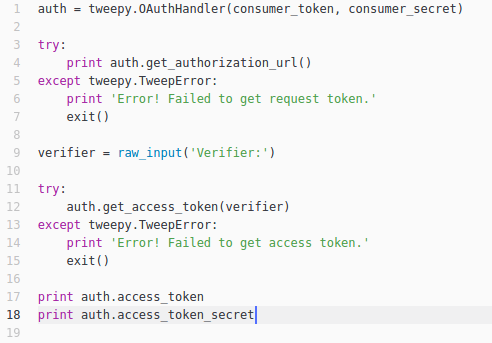
\includegraphics[width=\textwidth]{Images/Implementation/oauth}
    \caption{Twitter OAuth handshake} \label{fig:oauth}
\end{figure}

\subsubsection{Querying the API}
Once the access token and access token secret have been obtained, a Tweepy API object can be made, which allows the application to make queries to the Twitter API. This script can iterate over tweet IDs and retrieve tweets in order to collect their text, as shown in figure \ref{fig:get-tweets}. The output of the script can then be saved as the new dataset CSV, with tweet IDs replaced by their corresponding text.

\begin{figure}[H]
    \centering
    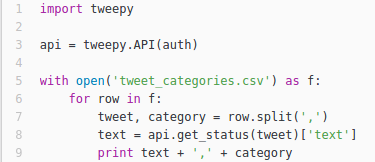
\includegraphics[width=\textwidth]{Images/Implementation/get-tweets}
    \caption{Get Tweet from API} \label{fig:get-tweets}
\end{figure}

\subsubsection{Virtual Private Servers}
Due to the size of the training set and the rate limits imposed by Twitter on their API, the amount of time it would take to process the entire original dataset to collect tweets would be significant. To mitigate this, multiple access tokens can be used simultaneously on separate Virtual Private Servers, by dividing the dataset amongst the servers and running the script remotely, since the rate limits are imposed on each access token rather than each application. For the purposes of this task, the CentOS Digital Ocean droplet was used ~\cite{DigitalOcean:Home}. Although the amount of storage on the droplet means that the entire dataset can not be processed - even when dividing amongst 10 access tokens - it allows a large enough dataset to be produced within a reasonable time frame.

\subsection{Template Data}
The template data required to populate the platform can be simply added to the Laravel database using the migration seeders. Figure \ref{fig:seed} shows the user seeder file, which adds the template data for the users table to the database through the \emph{User} model. Each attribute in the \emph{User} model corresponds with a column on the users table. To add the seeds into the table, the Artisan command \textit{php artisan db:seed} is executed.

\begin{figure}[H]
    \centering
    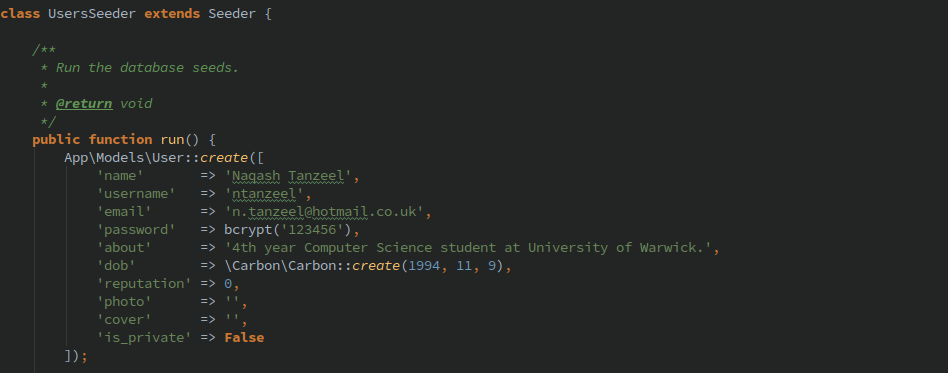
\includegraphics[width=\textwidth]{Images/Implementation/seed}
    \caption{User Seed} \label{fig:seed}
\end{figure}

\subsection{User Authentication}
The form shown in figure \ref{fig:register-page} is used to collect the data needed in order to authenticate access for the user, which includes the password fields and also the email address so that a password can be recovered in case it is forgotten by the user. When this form is submitted, the form data is passed to the \emph{RegisterController}, which handles adding the user to the database via the \emph{User} model. The function which performs this process is shown in figure \ref{fig:register-controller}.

\begin{figure}[H]
    \centering
    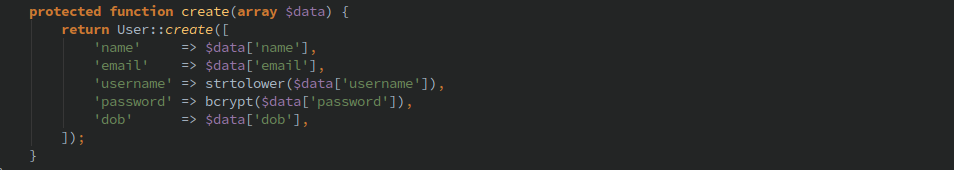
\includegraphics[width=\textwidth]{Images/Implementation/register-controller}
    \caption{Register Controller} \label{fig:register-controller}
\end{figure}